\chapter{Stacks}
Our next data structure is the Stack.
The stack may seem unnecessary as a data structure after we introduce its features.  
After all, can't a list do all the things that a stack can do and more? 

Working with the limited operations of a allows us to approach problems with a different mindset.

\section{Stack Operations}

The stack operations are limited and simple. 

\begin{enumerate}
	\item[\textbf{Push}] Put an item on the top of the stack.
	\item[\textbf{Pop}] Remove the item from the top of the stack and return it.  The item that was underneath the top of the stack becomes the new top.
	\item[\textbf{Peek}] Return the top of the stack, without removing it.
\end{enumerate}


That's it.  That's all there is.  It is refreshingly simple.
There will usually be additional functions, such as one to check if the stack is empty or a function to get the number of items stored in the stack, but \texttt{push}, \texttt{pop}, and \texttt{peek} are the important ones.


The common metaphor used for this is a stack of pancakes (Figure \ref{fig:pancakeai}).  You wouldn't remove a pancake from the bottom of the stack or the middle --- that would know over the whole stack! Instead, you move would only want to add or remove pancakes from the top of the stack.\footnote{I find the metaphor silly as that implies there's a situation I would willingly remove pancakes from my stack.}

\begin{figure}
	\centering
	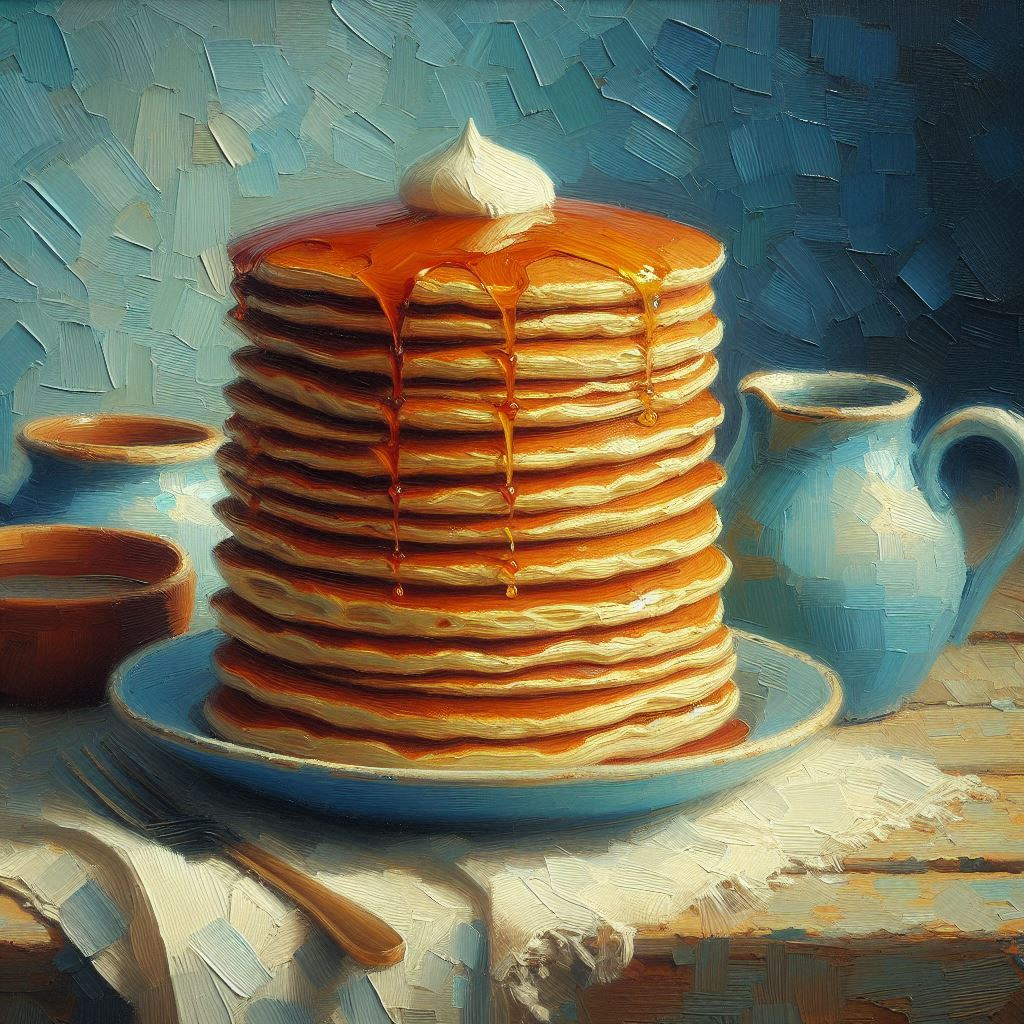
\includegraphics[width=0.7\linewidth]{pics/pancake_ai}
	\caption[AI Pancakes]{Delicious, AI-generated pancakes}
	\label{fig:pancakeai}
\end{figure}


\section{Building a Stack}

We will be building a stack as a reference-based structure in this book.  This is so we can get a bit more practice with manipulating nodes.


%https://runestone.academy/ns/books/published/pythonds3/BasicDS/ImplementingaStackinPython.html
	

\begin{javacode}{The Stack (Java)}
public class Stack<E> {
	private Node<E> top;
	
	public boolean isEmpty(){
		return top == null;
	}
	
	public E peek() {
		return top.item;
	}
	
	public E pop() {
		E toReturn =  top.item;
		top = top.next;
		return toReturn;
	}
	
	public void push(E item){
		Node<E> newTop = new Node<E>(item);
		newTop.next = top;
		top = newTop;
	}
	
	private static class Node<E>{
		E item;
		Node<E> next;
		public Node(E item) {
			this.item = item;
		}
	}	
}\end{javacode}


% converted the above code with chatGPT
% Then made edits to remove injected error messages
% and match style



\begin{pycode}{The Stack}
	
class Stack:
	class Node:
		def __init__(self, item):
			self.item = item
			self.next = None
	
	def __init__(self):
		self.top = None
	
	def isEmpty(self):
		return self.top is None
	
	def peek(self):
		return self.top.item
	
	def pop(self):
		toReturn = self.top.item
		self.top = self.top.next
		return toReturn
		
	def push(self, item):
		newTop = self.Node(item)
		newTop.next = self.top
		self.top = newTop
\end{pycode}


\section{Built-in Stacks}

Our programming languages have functionality for Stacks built into them, although it is different than our pedagogical model.
\subsection{The Stack - Java}
The built in \texttt{Stack} for Java uses an array-based\footnote{Stack is a subclass of the \texttt{Vector} class, itself a subclass of the \texttt{AbstractList} abstract class.  The \texttt{Vector} is extremely similar to \texttt{ArrayList} but older.  You should not use a \texttt{Vector} unless you have an extremely specific reason;  I have never had a reason.} implementation, rather than a reference based implementation, like above.  It uses all the conventional Stack

However, if you were to actually use a \texttt{Stack} in production, you should instead use a \texttt{Deque} according to the JavaDoc:
%TODO: CITE https://docs.oracle.com/javase/8/docs/api/java/util/Deque.html
``Deques can also be used as LIFO (Last-In-First-Out) stacks. This interface should be used in preference to the legacy \texttt{Stack} class. When a deque is used as a stack, elements are pushed and popped from the beginning of the deque.'' 
However, \texttt{Deque} uses a different naming system for its operations, rather that names like \texttt{push} ir \texttt{pop}.  As a result, \texttt{Deque} will be more briefly mentioned in Chapter \ref{chap-queue}'s coverage of Java's Queue, but it is worth the mention here. 
 
Conclusion, use \texttt{Stack} in this course, but be prepared to use \texttt{Deque} outside the course.


\subsection{The List - Python's Stack}
Python has no separate built-in stack. Rather, we instead use a  \href{https://docs.python.org/3/tutorial/datastructures.html#using-lists-as-stacks} {Rather, it uses the List that we are already familiar with} to emulate a stack\footnote{And the Queue, as we will see in Chapter \ref{chap-queue}} and operates on the last (right-most) index of the list.

If you want to use a Python list as a stack, merely restrict yourself to using the \texttt{append(item)} function in place of \texttt{push}.
Python lists have a \texttt{pop} method;  when called without any argument\footnote{When provided an index, \texttt{pop} removes and returns the item at that index.  
Python uses \texttt{pop} to remove at an index, whereas \texttt{remove} is used to remove and return the first occurrence a specified item.},  it removes and returns the last element in the list.

Use \texttt{stackname[-1]} to \texttt{peek} at the top of the stack.


\section{Why?}
Why use a stack over a much more powerful data structure?    Using stacks (and queues) help focus on seeing if there's a particular strategy for solving a problem.  With stacks, that strategy is typically backtracking.   Furthermore, limiting the operations of storing and retrieving data to operating on only the front/top of a list-like structure means that we can ensure all storage and retrieval operations run in $O(1)$ time.


\section{Mazes - Stacks and Backtracking}

If you haven't ever done a hedge maze, you should try it out.  They are pretty fun in my opinion and certainly doing at least once.  That said, I would venture most people playing in a maze of some sort meander through with a vague strategy, picking a direction they hope will get them closer to the goal.

Let me teach you two such strategies for when you get stuck in a maze.  The first strategy is the ``hand on wall'' rule or ``right hand'' rule.  It requires no preparation and works on almost every maze.  Simply take your right hand and lay it upon the wall of the corridor you are in.  Move forward and when you come to a turn, travel so that you never lift your hand off the wall.  So long as the entrance and exit are on the same wall (which they almost certainly are), you'll eventually make your way out.

The second strategy is backtracking\footnote{Technically this is going to look a lot like Depth First Search, but this is a very specific variation of it.} and works on any maze you are likely to encounter.\footnote{The exception is mazes that change their configuration while you are in them.}  Let's explore this using an example from Greek Mythology: the Labyrinth. 

% Greek mythology
\subsection{The Labyrinth}
Once upon a time, King Minos, child of Zeus and big jerk of a demigod, really messed up and angered Poseidon.  Minos's wife then gave birth to the Minotaur, a half-man/half-bull.  Minos had the inventor Daedalus build the Labyrinth for him to keep the Minotaur in.  The Labyrinth was a giant maze, and Minos, being a big jerk, frequently tossed Athenians into the Labyrinth to feed the Minotaur.  

This continued until Theseus, son of Poseidon, put a stop to it by navigating the Labyrinth and slaying the Minotaur. Theseus managed to pull this off with the help of Ariadne, Minos's daughter and noted not big jerk. Ariadne provided Theseus with a ball of thread, which allowed him to navigate the Labyrinth. Minos eventually died in a bizarre series of events involving him being a stalker, a seashell, and even more thread.

It's the thread here that we are concerned with.  See, the Labyrinth is classically understood to have a ton of twists and turns and easy to get lost in.  Let's put ourselves in the shoes of Theseus for a second and think about how we can use that thread to navigate this maze.  

Since we're pretending we're a demigod protagonist of a Greek myth, we might as well pretend that Ariadne's thread is magic too.  We won't run out of thread and it can't be cut by the Minotaur or otherwise tangled.  Let's also assume we're in one of the versions of the myth where we have a sword. We will let the thread unroll along the ground as a we traverse the maze.  When we come to a crossroads or some other choice of passages, we will travel down an unexplored passage.  


It's possible we hit a dead end in one of two ways.  The first way we hit a dead end is that the corridor ends;  a literal dead end.  The second way we can hit a dead end is by coming to a crossroads and there are no unexplored passages.  In either case, we can backtrack.

To backtrack, we turn around and follow the thread until we find an unexplored passage.  We wind the thread back up and mark the floor or walls with the sword to let our future selves know this was a dead end \footnote{If we don't have a sword, we don't wind the thread back up, because if we did, we'd end up essentially erasing markers we have that a passage has been explored. Instead, we will leave a second line of thread along the ground on passages we backtrack upon.  We have the sword for pedagogical reasons, a sentence I never thought I would write, but always hoped that I would.}. We know we have found an unexplored passage when find a passage with no thread or sword marks. This will allow us to navigate the entire maze and ensure we only ever traverse a passage twice:  once while exploring and once while backtracking.


Abstracting this out, each corridor (or cell of the maze when we get programming) has three states:

\begin{description}
	\item[Unexplored] This is a part of the maze we haven't traveled down yet.
	\item[Visited] This would be part of the maze we have traversed.
	\item[Backtracked] This is a part of the maze we have traversed \textit{twice}, the second time being us reversing our trail.
\end{description}

We can use a Stack in place of our magic thread, using the \texttt{push} operation on a location to say we have traveled to this location, with the top of the Stack holding our current location.  This is analogous to unrolling the thread. If we need to backtrack, we \texttt{pop()} and go to the location that's now at the top of the task.  This represents the act of us rolling the thread back

Rather than awesome sword, we will use much more mundane \texttt{booleans} or \texttt{enums} or \texttt{colors} to ensure we don't revisit an already explored or backtracked corridor.  Which we use depends on our implementation.


This gives us our algorithm.

\begin{verbatim}
Given: a maze represented by a 2D array of cells
Cell: represents a unit of the maze. 
    Has a variable for color or exploration status.
    Also has variables to represent walls or lack thereof
    in each of the cardinal directions

Algorithm:
push start position on top of stack
while maze exploration is not done and and stack isn't empty
    peek at the stack to get our current position
    if we can go north and haven't visited there yet
        push the location to the north on the stack
        mark the current location as visited
    else if we can go south...
    repeat for east and west
    else
    we can't go anywhere so we are at a dead end
        mark current as a dead end
        pop off the stack
\end{verbatim}


We can assume that maze exploration is done if we find the exit.  If the stack is empty, we have come back to the beginning of the maze.  
The last note I'll make before our next topic is possibly the most intriguing.  With a bit of creativity and some minor tweaks, we can take this algorithm and modify it to \textit{generate} mazes rather than solve them. Generating mazes is it's own fun subgenre, as each strategy and algorithm for creating mazes creates mazes with different biases. 


\section{Parenthesis Matching}

A classic stack problem is to write a program that checks to see if a given string has balanced parenthesis.  As a student, you encounter this problem in three places: a data structures class like this, an interview question, or Computer Automata class.\footnote{This problem is used to show the limits of Discrete Finite Automata/Regular Languages and introduce Stack Machines/Context Free Grammars}
The question we're trying to answer is something like ``Does the string \texttt{ ((A + f(x[0])) + B} have balanced parentheses?''  We humans can easily take a look and say no, \texttt{ ((A + f(x[0])) + B} doesn't balanced parentheses; it's missing a closing parenthesis.  But how did we do that?  Codifying that is how we solve this problem.  

Now if it was a matter counting the number of opening and closing parenthesis, this would be an easy problem.  But in asking if the parenthesis are balanced, we're essentially asking if they match in a way that makes mathematical sense: everything is nested correctly; nothing closed before it opens. Simply counting the correct number of opening and closing parenthesis would fail on \texttt{a)(} and \texttt{fx)())}.

Instead, we can use a specific tool to handle this problem.  If you guessed it is the stack, excellent work.  You must have caught on to the numerous hints, such as this being in the chapter about stacks, or the starting sentence talking about how this is a classic stack problem.

We parse thru the string and skip anything not a parenthesis or bracket or the like.  When we see an open parenthesis/bracket, we push it onto the stack.  When we see a closing brace, we pop from the stack and compare. If we have a match, no issues.  But if the type of brace or bracket or parenthesis doesn't match or there was nothing to pop off, return false.

\begin{javacode}{Parenthesis Matching in Java}
public static boolean isBalanced(String expression) {
	Stack<Character> stack = new Stack<>();
	for (Character c : expression.toCharArray()) {
		if(c == '(' || c=='[' || c == '{' ) {
				stack.push(c);
				
			} else if( c== ')' || c== ']' || c == '}') {
			if(stack.isEmpty()){
				return false;
			}
			char opener = stack.pop();
			if( !((opener=='(' && c==')') || (opener=='[' && c==']') || (opener=='{' && c=='}'))){
				return false;
			}
			
		}
		
	}
	return stack.isEmpty();
}


\end{javacode}

\begin{pycode}{Parenthesis Matching in Python}
def isBalanced(expression):
	stack = []
	for c in expression:
		if c in "([{":
			stack.append(c)
		elif c in ")]}":
			if not stack:
				return False
	opener = stack.pop()
	if not ((opener == '(' and c == ')') or 
			(opener == '[' and c == ']') or 
			(opener == '{' and c == '}')):
		return False
	return not stack
\end{pycode}
%\section{Discrete Finite Automata}
